\documentclass[conference]{IEEEtran}

\usepackage[numbers]{natbib}
\usepackage{graphicx}
\usepackage{amsmath}
\usepackage{amssymb}
\usepackage{amsthm}

\newtheorem{lem}{Lemma}
\newtheorem{Hyp}{Assumption}
\newtheorem{propty}{Property}
\newtheorem{thm}{Theorem}
\newtheorem{mydef}{Definition}

\usepackage{algorithm}
\usepackage{algorithmic}
\renewcommand{\algorithmicrequire}{\textbf{Input:}}
\renewcommand{\algorithmicensure}{\textbf{Output:}}

\usepackage{subfigure}
\usepackage{float}

\begin{document}

\title{Informative Path Planning with a Human Path Constraint}

\author{
\IEEEauthorblockN{Daqign Yi, Michael A. Goodrich and Kevin D. Seppi}
\IEEEauthorblockA{Department of Computer Science\\
Brigham Young University\\
Provo, Utah 84604\\
Email: daqing.yi@byu.edu, \{mike, kseppi\}@cs.byu.edu}
}

\maketitle

\begin{abstract}
One way for a human and a robot to collaborate on a search task is for the human to specify constraints on the robot's path and then allow the robot to find an optimal path subject to these constraints.
This paper presents an anytime solution to the robot's path-planning problem when the human specifies a path constraint and an acceptable amount of deviation from this path.
The robot's objective is to maximize information gathered during the search subject to this constraint.
We first discretize the path constraint and then convert the resulting problem into a multi-partite graph.
Information maximization becomes a submodular orienteering problem on this topology structure.
Backtracking is used to generate an efficient heuristic for solving this problem, and an expanding tree is used to facilitate an anytime algorithm.
\end{abstract}

\IEEEpeerreviewmaketitle

\section{Introduction}
\label{sec:intro}

This project is based on ``Distributed cooperative attitude synchronization and tracking for multiple rigid bodies'' by Dr. Ren \cite{5229134}, in which discusses the consensus seeking of a system of agents with non-linear model.
Two approaches have been proposed for ``cooperative attitude synchronization'' (position control) and ``reference attitude tracking'' (trajectory tracking) respectively.
Two approaches are stated independently and look different.
One objective of this project is seeking the consensus between two approaches, which can be used as a pattern on analyzing other synchronization systems and designing control laws for them.

The structure of this report is as following.
Section \ref{sec:prob_stat} states the system model, which includes the rigid body dynamics of each agent and the interaction topology.
Section \ref{sec:coop_att_syn} presents the control law proposed for the cooperative attitude synchronization and the proof strategy.
%I try to figure out the roles of the terms in the control law so that I can simplify the control law with ignorance on the transient performance and prove the stability.
By analyzing the roles of the terms in the control law, I simplify the control law to find the essential component that guarantees the stability.
It means that the stability can still be preserved and proved without some terms for transient performance.
Section \ref{sec:ref_att_trk} illustrates the control law proposed for the reference attitude tracking and the proof strategy.
I use a same proof strategy to prove the stability of the control law on the cooperative attitude synchronization, which shows the consistency between two approaches.
It means that the ideas of improvement can be applied to both control approaches.
Simulations are also taken on both approaches for analysis purpose.
Section \ref{sec:io_stable} proposes an interconnection perspective for analyzing a class of distributed system control problems as a pattern of analyzing a consensus-seeking problem.
A hypothesis on proving the stability is proposed, in which the proof can be achieved by analyzing the stability-relevant properties of the sub-components.
Section \ref{sec:summary} discusses some possible future work from Dr. Ren's paper.

\section{Problem definition}

\subsection{Informative path}

\begin{frame}{Coverage model}{Informative path}

\begin{itemize}
\item Maximum coverage problem
\item Information gain - entropy 
\end{itemize}

\begin{figure}
\centering
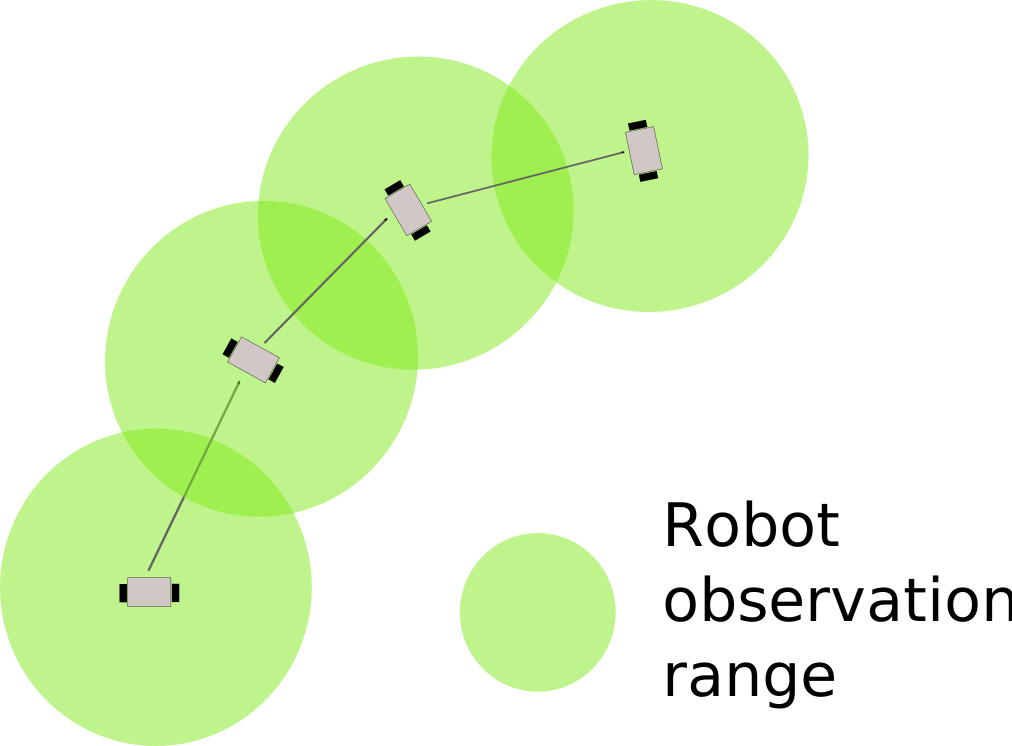
\includegraphics[width = 0.6\textwidth]{./figure/robotObservation}
%\caption{A coverage model.}
\end{figure}

\end{frame}

\begin{frame}{Submodularity}{Informative path}

\begin{columns}

\column{0.45\textwidth}

\begin{figure}
\centering
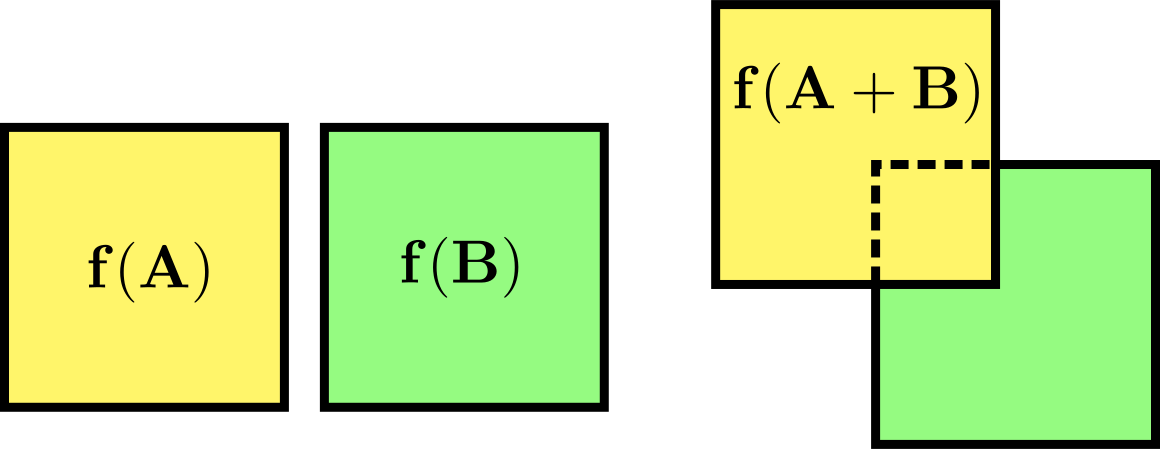
\includegraphics[width = \textwidth]{./figure/submodular}
%\caption{A coverage model.}
\end{figure}

\begin{equation}
\nonumber
f(A) + f(B) \geq f(A+B)
\end{equation}

\column{0.1\textwidth}

\column{0.45\textwidth}

Information
\begin{itemize}
\item search space $ S $
\item the observation of a robot $ \mathbf{O}^{X} $ 
\item the observation of a human $ \mathbf{O}^{Y} $

\bigskip
\bigskip

$ f( \mathbf{S}, \mathbf{O}^{X} ) + f( \mathbf{S}, \mathbf{O}^{Y^{h}} ) \geq f( \mathbf{S}, \mathbf{O}^{X},  \mathbf{O}^{Y^{h}} ) $ 
\end{itemize}

\end{columns}

\end{frame}

\begin{frame}{Submodular orienteering}{Informative path}

\begin{block}{Conditional mutual information}
$ I(\mathbf{S}; \mathbf{O}^{X} \mid \mathbf{O}^{Y^{h}}) = H(\mathbf{S} \mid \mathbf{O}^{Y^{h}}) - H(\mathbf{S} \mid \mathbf{O}^{X},\mathbf{O}^{Y^{h}}) $
\end{block} 

\bigskip

\begin{itemize}
\item Entropy reduction
\item Submodularity
\item Chain rule \\
$ I(\mathbf{S}; \mathbf{O}^{X} \mid \mathbf{O}^{Y^{h}}) = \sum_{t=1}^{T} I(O^{X}_{t} ; \mathbf{S} \mid O^{X}_{1} , \cdots , O^{X}_{t-1}, \mathbf{O}^{Y^{h}}) $
\end{itemize}

\end{frame}

\subsection{Human constraint}

\begin{frame}{Team role}{Human constraint}

\begin{figure}
\centering
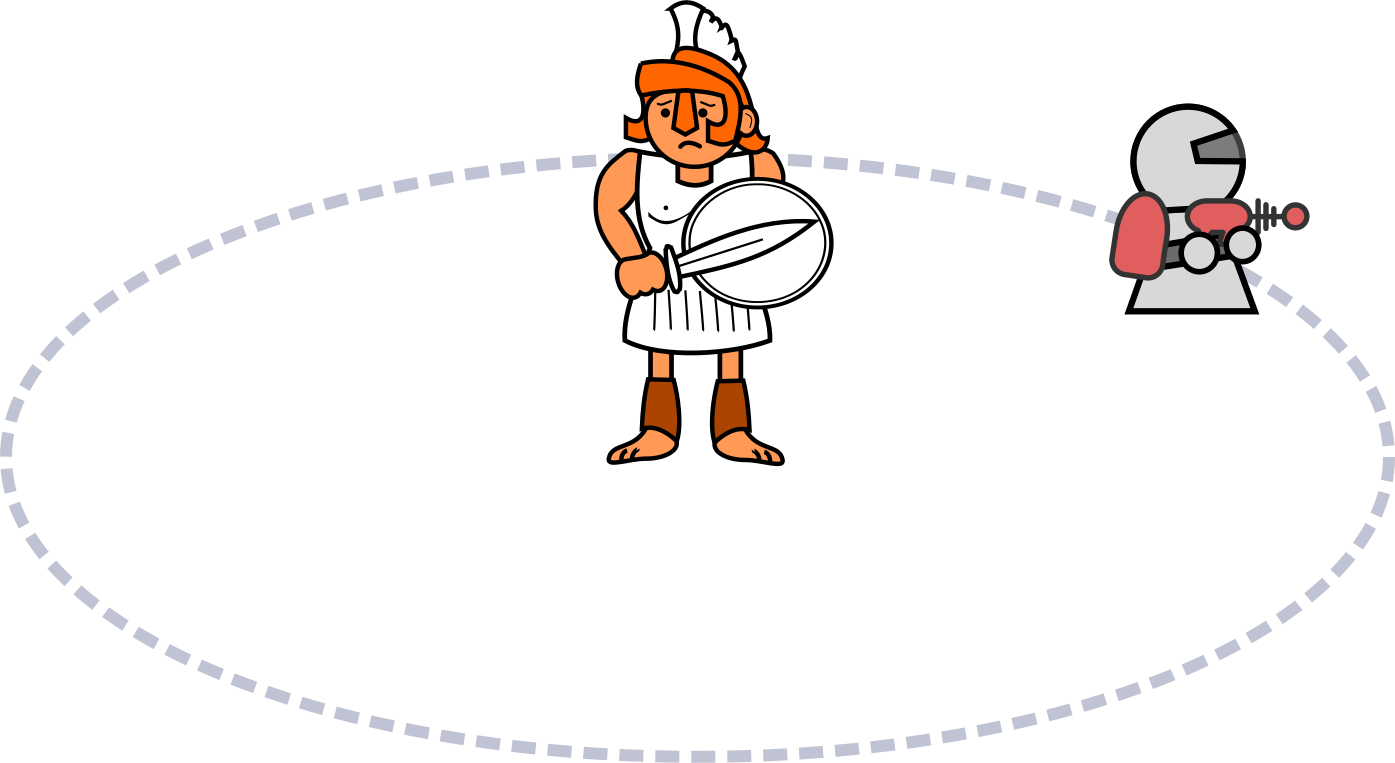
\includegraphics[width = 0.7\textwidth]{./figure/human_robot_interaction}
\end{figure}

\begin{itemize}
\item cooperative observation
\item assistance and protection
\end{itemize}

\end{frame}

\begin{frame}{Neighboring function}{Human constraint}

\begin{columns}
\column{.6\linewidth}
\begin{minipage}[c]{\linewidth}
\begin{figure}
\centering
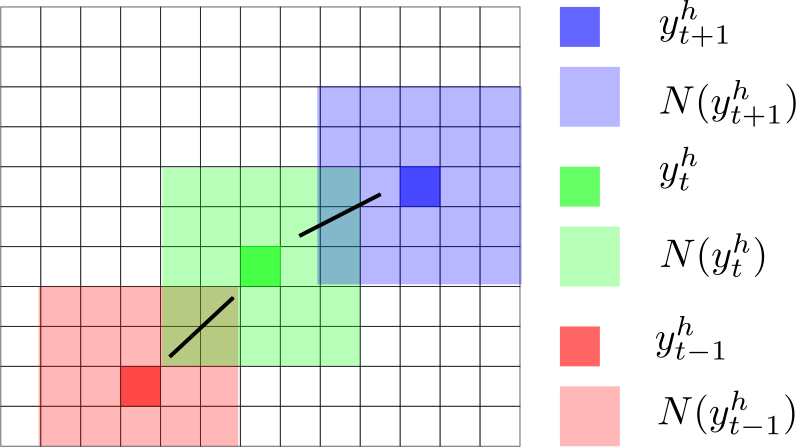
\includegraphics[width = \textwidth]{./figure/humanConstraint}
%\caption{An example of human constraint.}
\end{figure}
\end{minipage}

\column{.4\linewidth}
\begin{minipage}[c]{\linewidth}
\begin{itemize}
\item { human path $ \{ y^{h}_{1} \cdots y^{h}_{T} \} $ }
\item { neighboring function $ N( y^{h}_{t} ) $ }
\end{itemize}
\end{minipage}
\end{columns}

\end{frame}

\subsection{The optimization model}

\begin{frame}{Problem abstraction}{The optimization model}

\begin{figure}
\centering
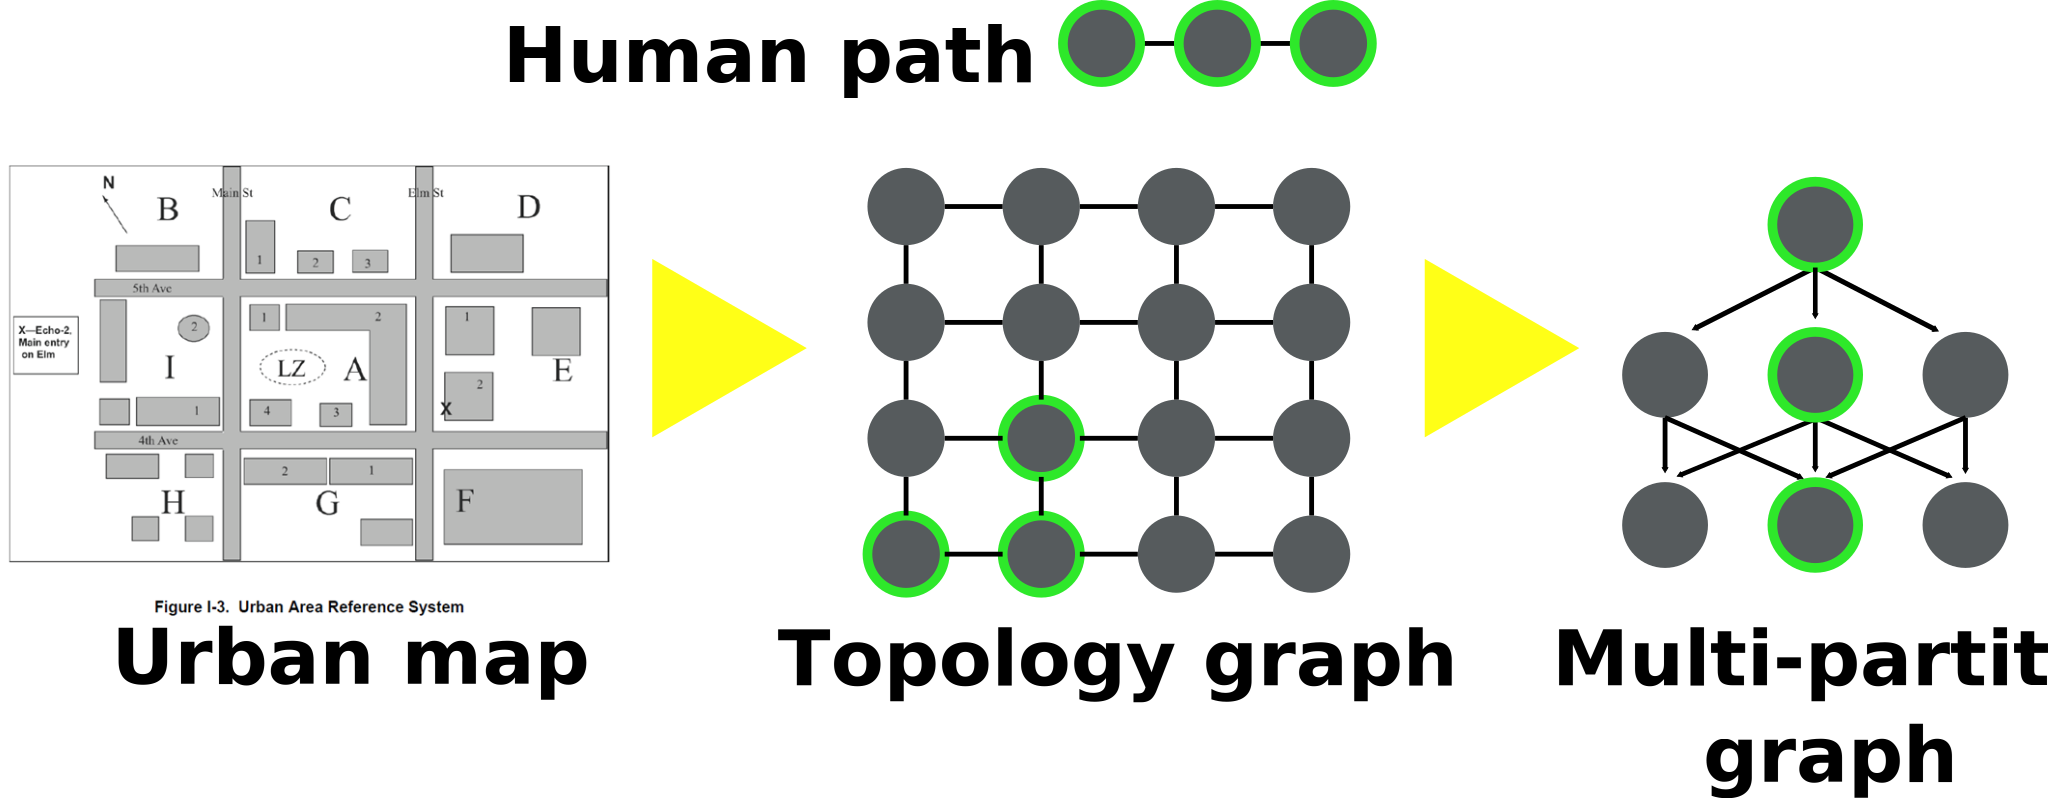
\includegraphics[width = 0.9\textwidth]{./figure/layers}
%\caption{A layered problem processing.}
\end{figure}

\end{frame}

\begin{frame}{The multi-partite graph}{The optimization model}

\begin{columns}

\column{.6\textwidth}
\begin{minipage}[c]{\linewidth}
\begin{figure}
\centering
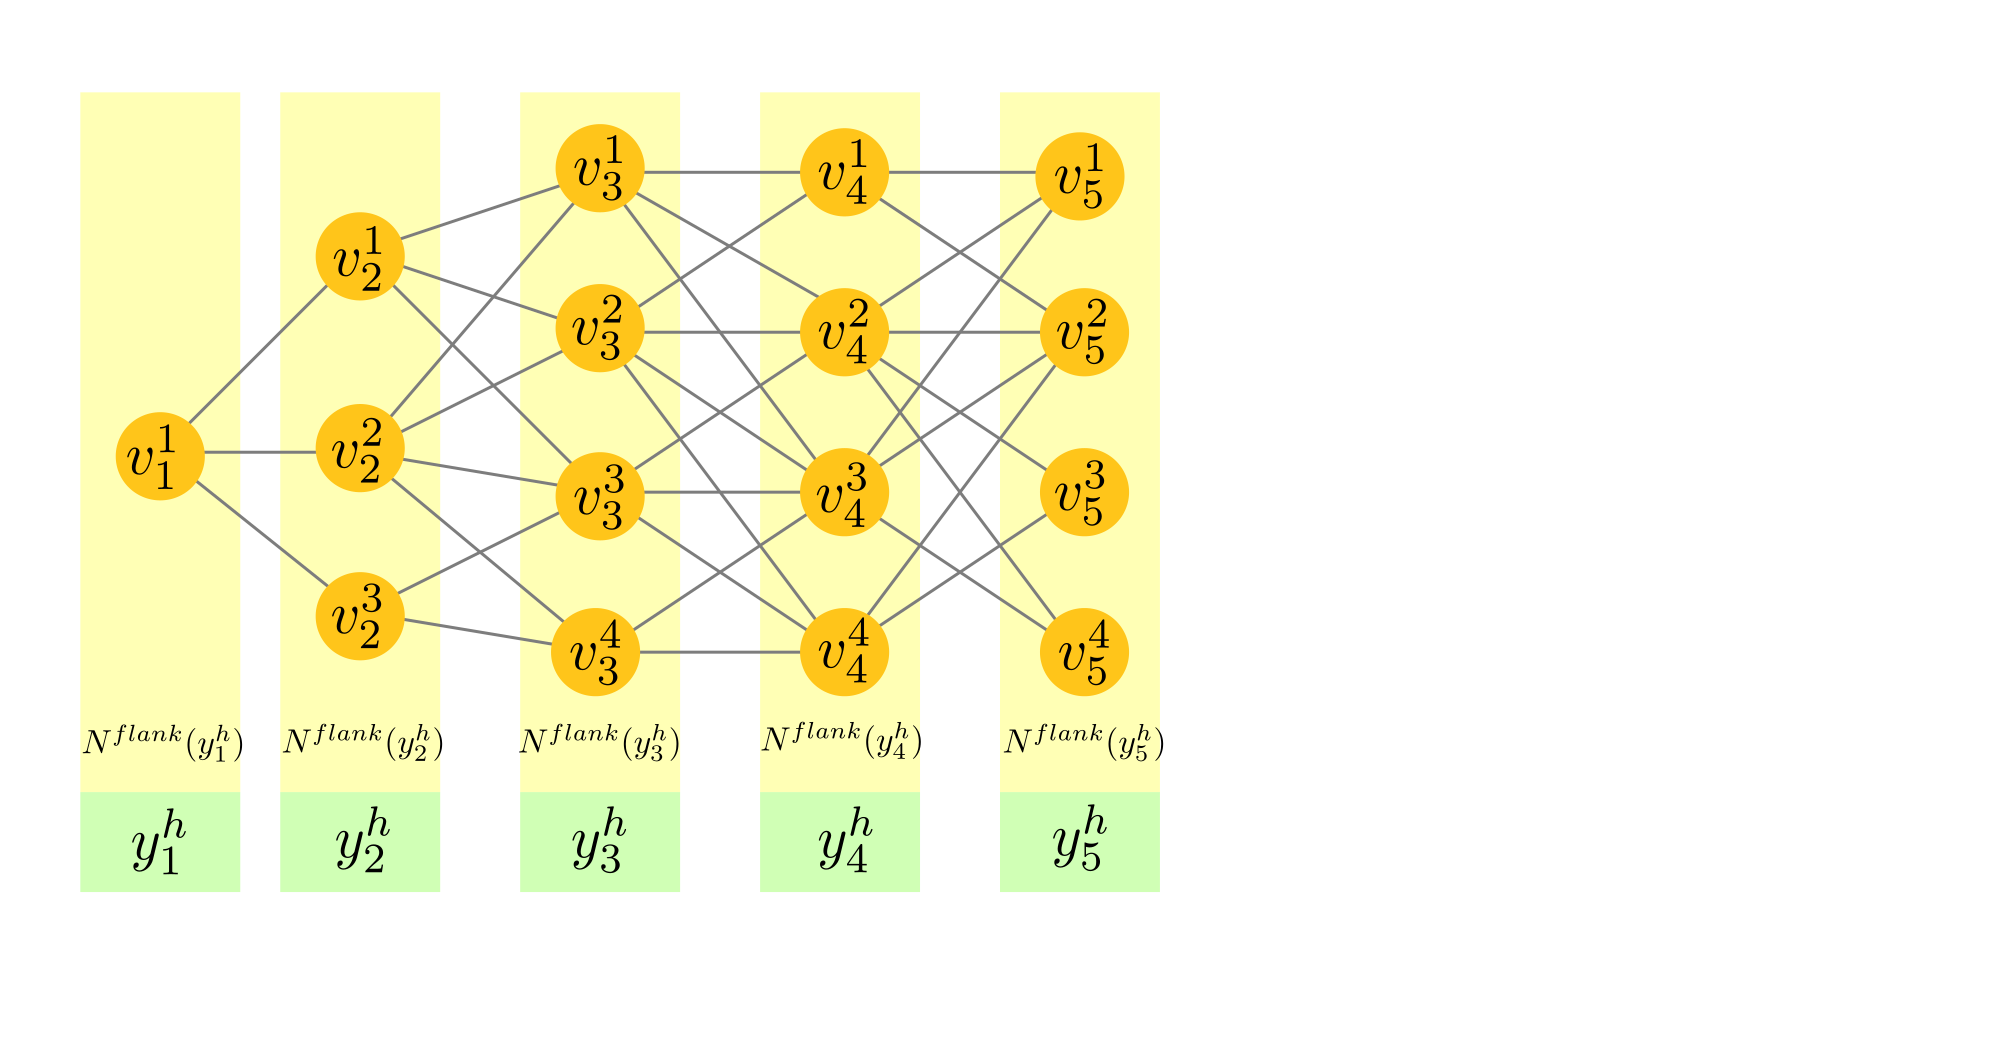
\includegraphics[width = 0.9\textwidth]{./figure/MultiPartite}
%\caption{A multi-partite graph generated from human constraint.}
\end{figure}
\end{minipage}

\column{.4\textwidth}
\begin{minipage}[c]{\linewidth}
%Multi-partite graph\\
%$ G = (V, E, T) $ 
%\begin{itemize}
%\item $ T $ - partition number
%\item $ V = \cup_{t=1}^{T} V(t) $
%\item $ (v^{i}_{t}, v^{j}_{t+1}) \in E $
%\end{itemize}
\end{minipage}

\end{columns}

\end{frame}

\begin{frame}{A pruning process}{The optimization model}

\begin{columns}

\column{.45\textwidth}

\begin{block}{Forward pruning}

Reachable

$ \forall t \in \{ 2, \cdots T \}, $ \\
$ \forall v \in V(t), deg^{-}(v) > 0 $

\begin{figure}
\centering
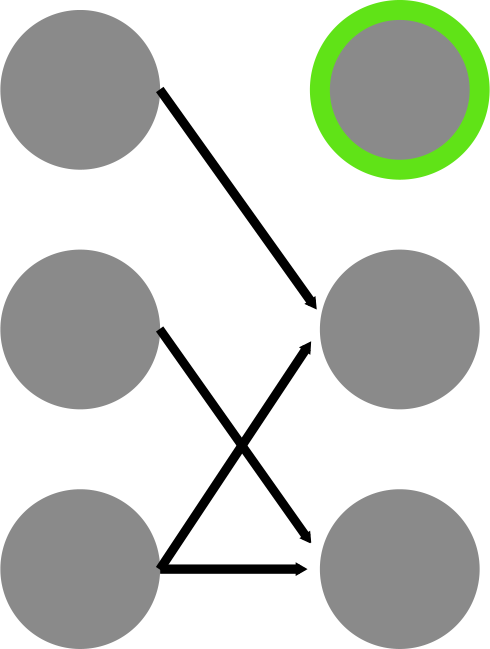
\includegraphics[width = 0.4\textwidth]{./figure/forward_prune}
\end{figure}

\end{block}

\column{.45\textwidth}

\begin{block}{Backward pruning}

Non-terminating 

$ \forall t \in \{ 1, \cdots T-1 \}, $ \\
$ \forall v \in V(t), deg^{+}(v) > 0 $


\begin{figure}
\centering
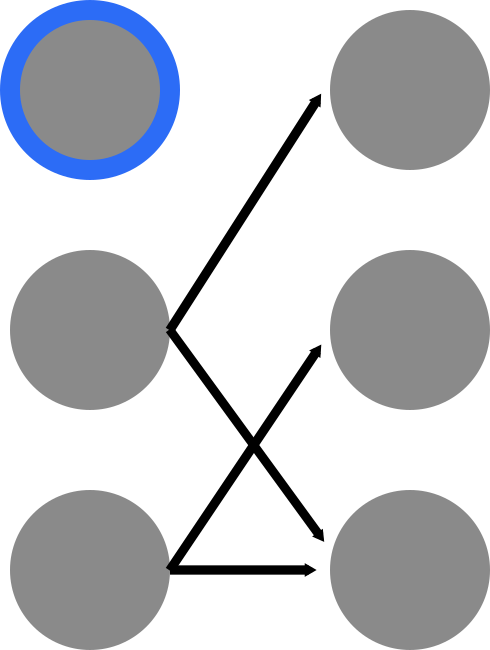
\includegraphics[width = 0.4\textwidth]{./figure/backward_prune}
\end{figure}

\end{block}

\end{columns}

\end{frame}

\begin{frame}{Obstacles}{The optimization model}

\begin{figure}
\centering
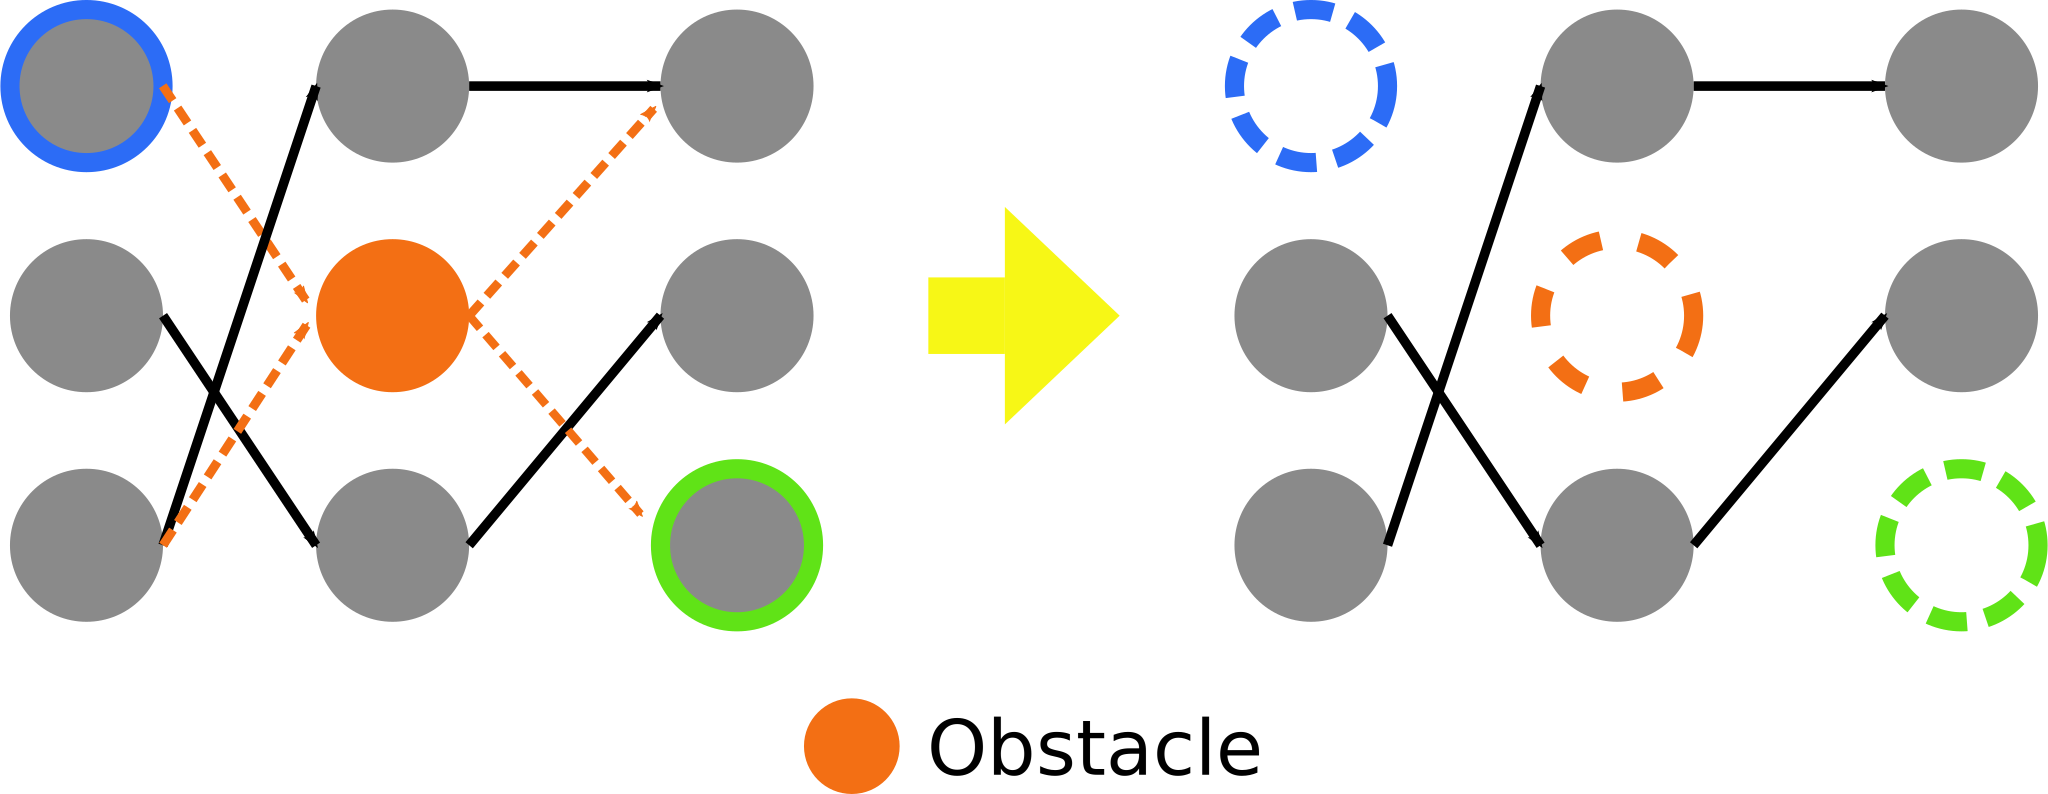
\includegraphics[width = 0.8\textwidth]{./figure/obstacle}
\end{figure}

\end{frame}

\begin{frame}{Submodular orienteering on a multi-partite graph}{The optimization problem}

\begin{equation}
\nonumber
\begin{aligned}
Objective: & X^{*} = \argmax_{X} \: f(X); \\
Constraint: & |X| = T, x_{t} \in V(t), (x_{t}, x_{t+1}) \in E.
\end{aligned}
\end{equation}

\end{frame}



\section{Solution}

\subsection{Backtracking heuristic}

\begin{frame}{Bellman-like equation}{Heuristic}

%\begin{equation}
%\nonumber
%\hat{x}_{t} = \argmax_{X_{t}} [ f(x_{t} \mid x_{1} , \cdots , x_{t-1}) + \max_{X_{t+1}, \cdots , X_{T}} f(x_{t+1}, \cdots , x_{T} \mid x_{1}, \cdots , x_{t}) ]
%\end{equation}

\centering
\includegraphics[width = \textwidth]{./figure/arg_equation}

\begin{columns}
\column{0.45\textwidth}
\begin{block}{Maximum future reward}
\begin{figure}
\centering
\includegraphics[width = 0.9\textwidth]{./figure/DefineFuncH}
\end{figure}
\end{block}

\column{0.45\textwidth}
\begin{block}{Maximum total reward}
\begin{figure}
\centering
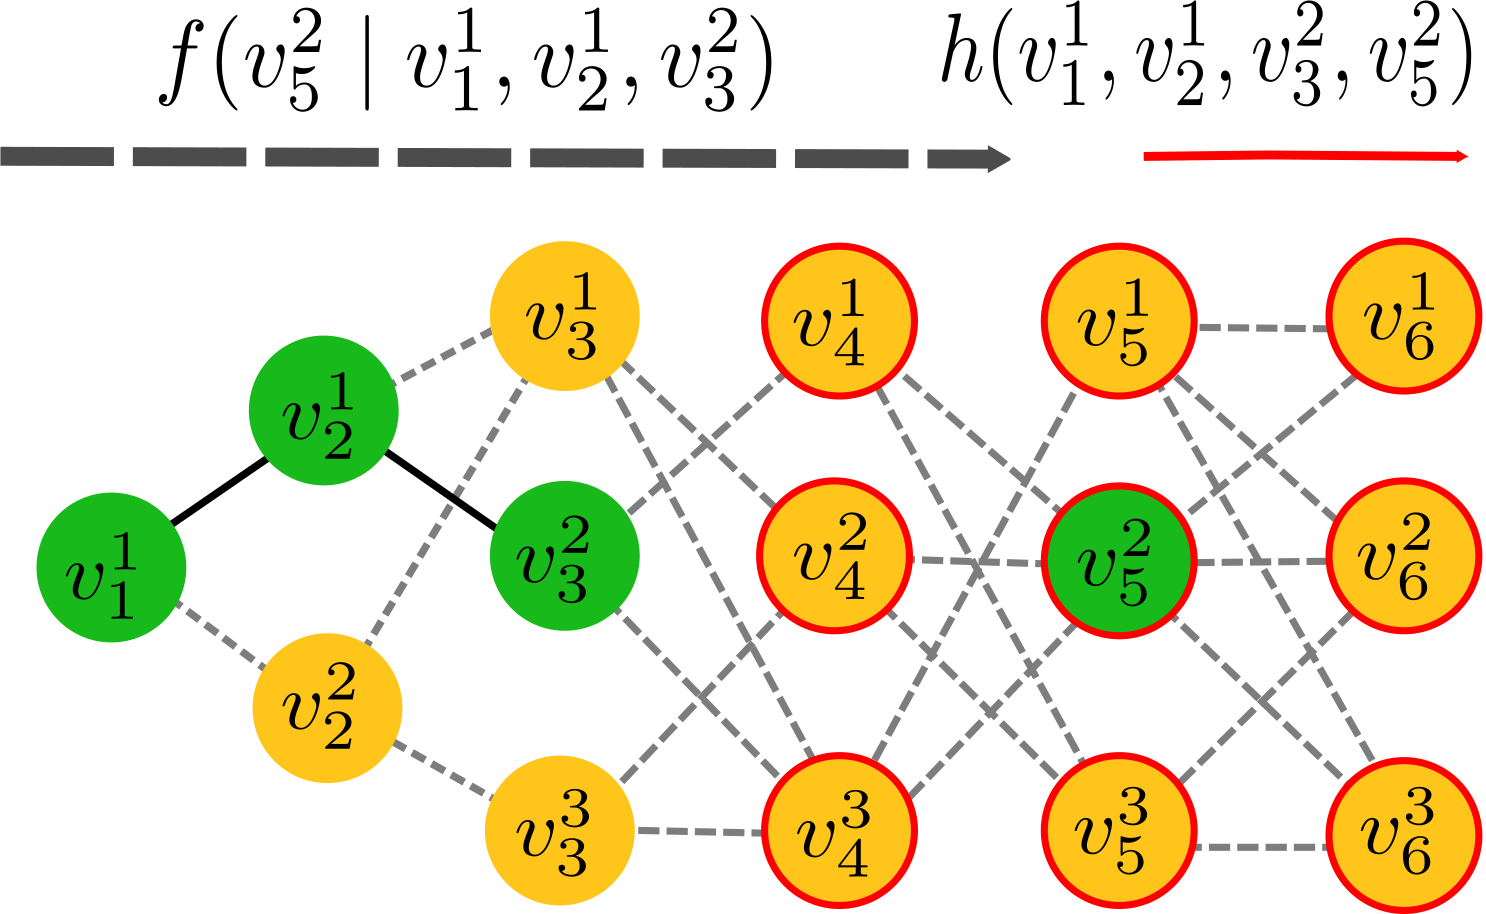
\includegraphics[width = 0.9\textwidth]{./figure/DefineFuncP}
\end{figure}
\end{block}
\end{columns}

\begin{figure}
\centering

\includegraphics[width = 0.9\textwidth]{./figure/DefineFuncHelp}
\end{figure}

\end{frame}

\begin{frame}{Backtracking}{Heuristic}

\begin{columns}

\column{0.6\textwidth}
\begin{minipage}{\textwidth}
\begin{figure}
\centering
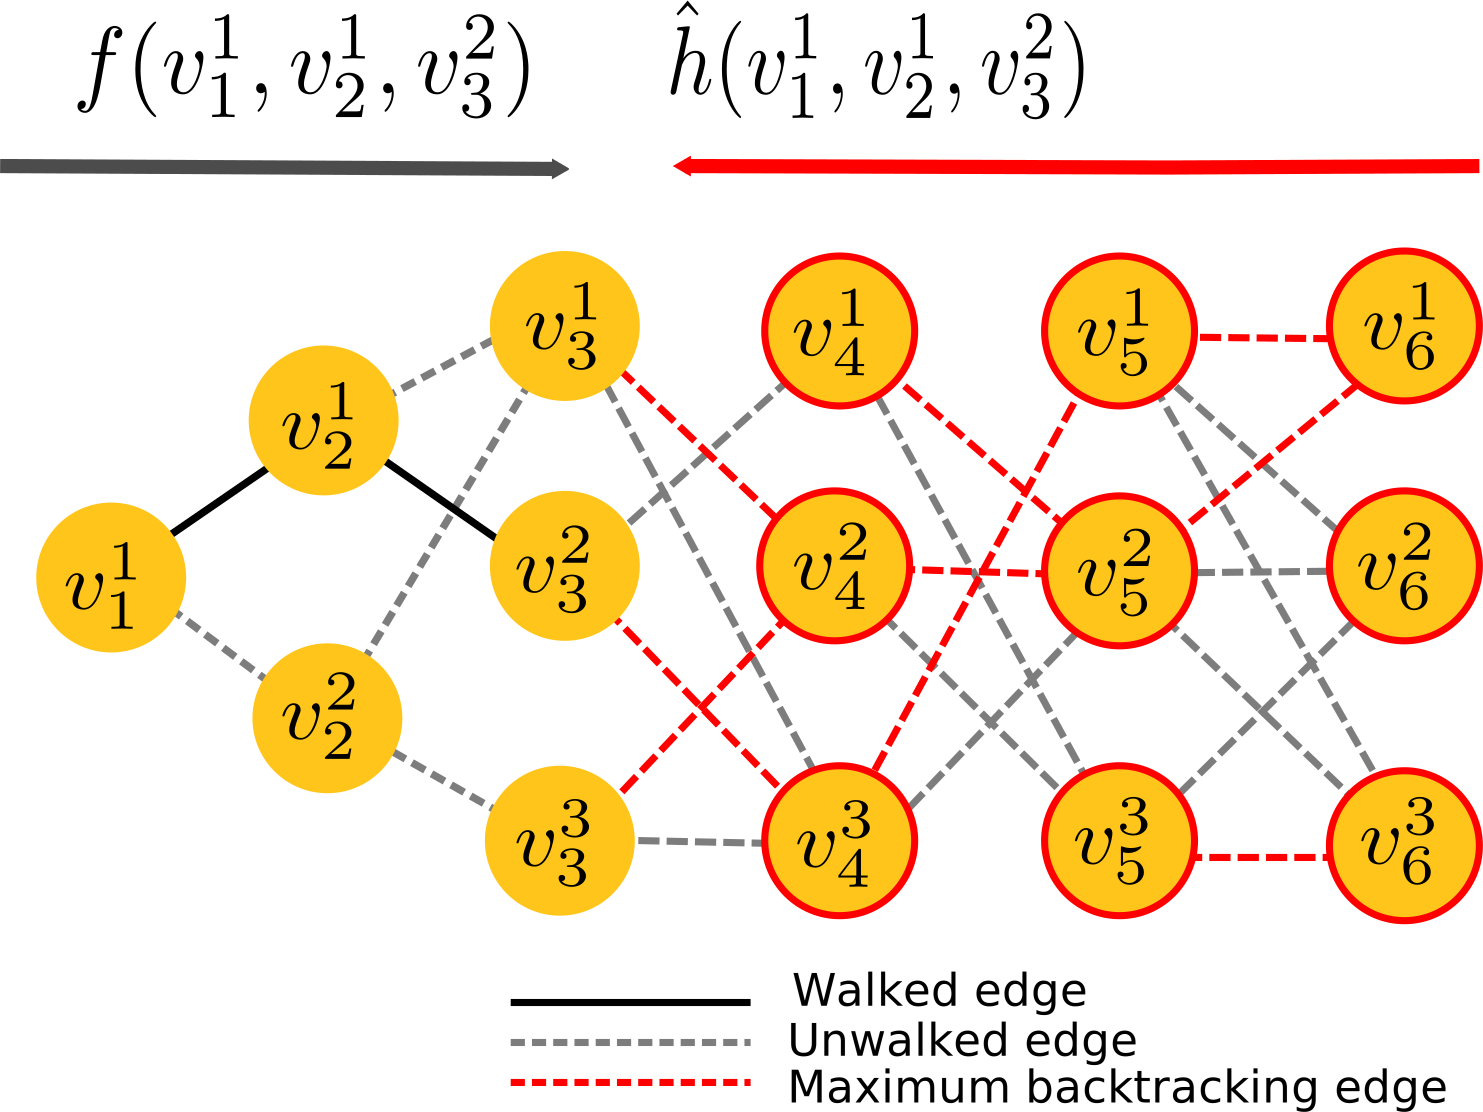
\includegraphics[width = \textwidth]{./figure/backtracking}
\end{figure}
\end{minipage}

\column{0.4\textwidth}
\begin{minipage}{\textwidth}
\begin{itemize}
\item point model $ \rightarrow $ true max total reward
\item coverage model $ \rightarrow $ estimated max total reward guarantee
\end{itemize}
\end{minipage}

\end{columns}

\end{frame}

\subsection{Anytime algorithm design}

\begin{frame}{Expanding tree}{Anytime algorithm framework}

\begin{columns}

\column{0.6\textwidth}
\begin{minipage}{\textwidth}
\begin{figure}
\centering
\includegraphics[width=.9\textwidth]{./figure/multipartite_expandingtree}
\end{figure}
\end{minipage}

\column{0.4\textwidth}
\begin{minipage}{\textwidth}
\begin{itemize}
\item depth-first recursive traverse
\item node $ \Longleftrightarrow $ subpath
\item tracking the search process
\item estimation storage
\end{itemize}
%Exapnding tree $ G_{T} = (N, L, T) $ \\
%\begin{itemize}
%\item $ T $ - tree depth
%\item $ N $ - Node set
%\item $ L $ - directed link set
%\end{itemize}
\end{minipage}

\end{columns}

\end{frame}

\begin{frame}{Node freeze}{Anytime algorithm framework}

Estimated reward $ \leq $ Current best reward 
$ \Longrightarrow $ Stop exploring subpath

\begin{figure}
\centering
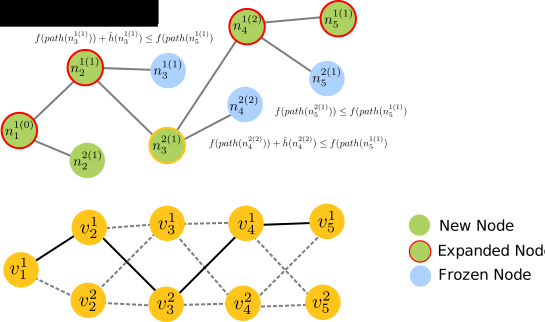
\includegraphics[width =  0.8\textwidth]{./figure/freeze_process}
\end{figure}

\end{frame}

\begin{frame}{Flow}{Anytime algorithm framework}

\begin{figure}
\centering
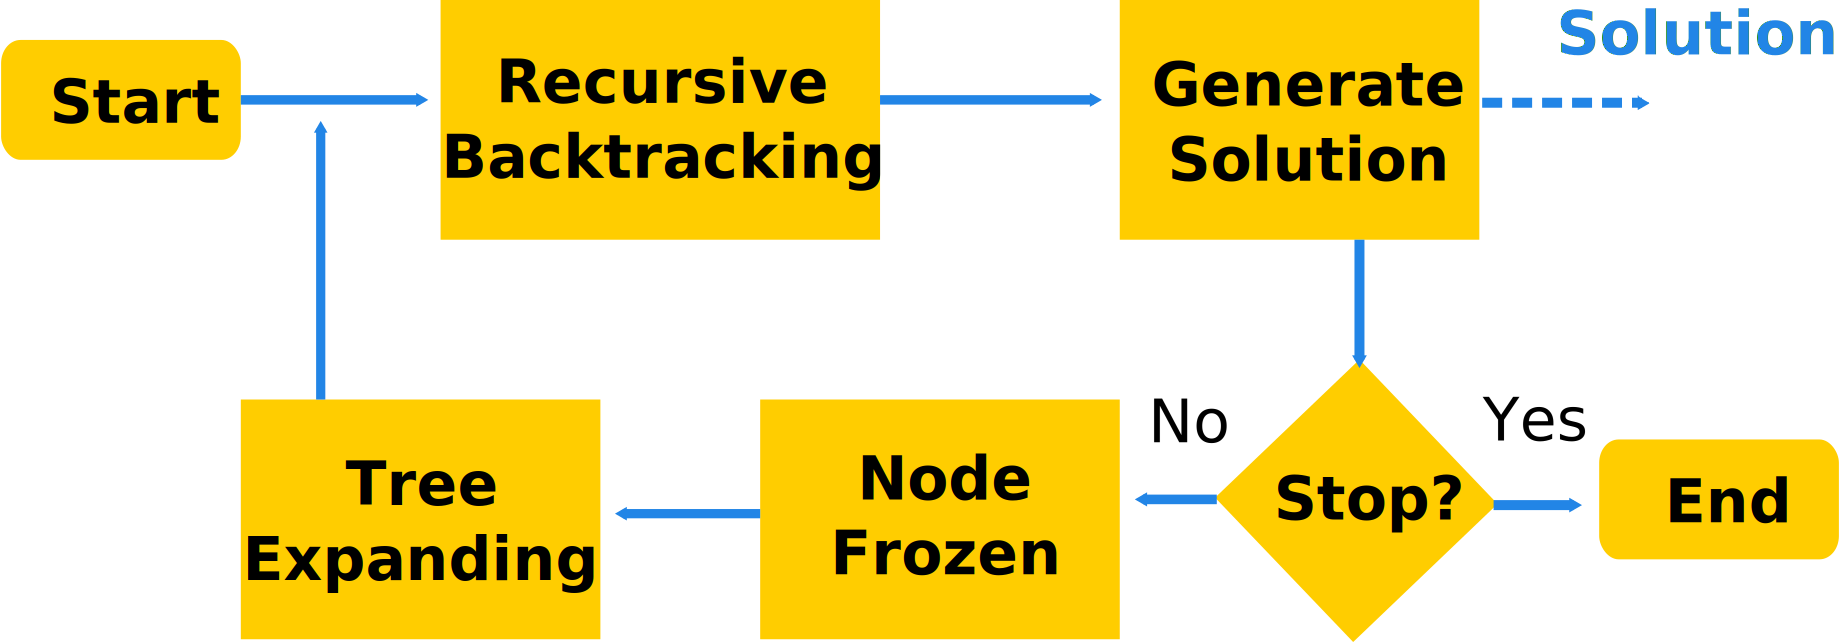
\includegraphics[width = 0.9\textwidth]{./figure/alg_flow}
\end{figure}

\end{frame}

\begin{frame}{Performance guarantee}{Anytime algorithm framework}

\begin{lemma}
“Backtracking” in Algorithm 1 never \textcolor{red}{underestimates}
the maximum total reward, which means
\begin{equation}
\nonumber
\forall t \geq t', \hat{u}(x_{t} \mid v_{1} , \cdots , v_{t'}) \geq u(x_{t} \mid v_{1} , \cdots , v_{t'}).
\end{equation}
\end{lemma}

\begin{minipage}{\textwidth}
\begin{figure}
\centering

\includegraphics[width = 0.15\textwidth]{./figure/arrow}
\end{figure}
\end{minipage}

\begin{theorem}
The anytime algorithm framework in Algorithm 4 can always find an \textcolor{red}{optimal} solution given enough time.
\end{theorem}

\end{frame}

\section{An Application to Robot Wingman}
\label{sec:wingman}

In this section, we apply Algorithm \ref{alg:Anytime} to the robot wingman problem~\cite{goodrich2013toward}.
Let $R_{\rm flank}$ denote the {\em flank support range}, which determines the area that a robot wingman is expected to stay in when a human is moving; this is illustrated in Figure \ref{fig:Wingman}.
The robot wingman constraint requires that $ \forall t, || x_{t} - y^{h}_{t} || \leq R_{flank} $ or, equivalently, 
$ \forall t \in T,  x_{t} \in N( y^{h}_{t} ) $.

Consider a two-dimension search space discretized into a world of hexagonal cells.
This discretization gives a constant distance from the center of one cell to any of its immediate neighbors, which facilitates modeling the agent observation range.
Moreover, a hexagonal tessellation is consistent with the assumption that we made that the robot would move at constant speed from one cell to another; in a hexagonal tessellation, the distances between the centers of all neighboring cells and the current cell is constant.

\begin{figure}
\centering
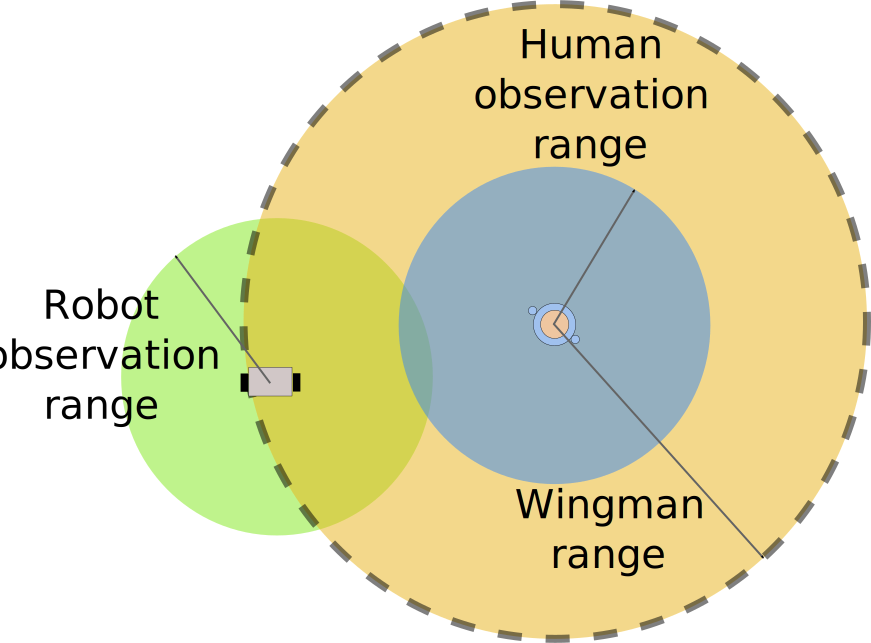
\includegraphics[width=0.35\linewidth]{./images/Wingman.pdf}
\caption{A Robot Wingman Framework.}
\label{fig:Wingman}
\end{figure}

The observation model of an agent uses the likelihood of detecting an object of interest in cell $ i $ and follows Bayes rule in updating the posterior~\cite{goodrich2013toward}.
Since we know the human's path, $ Y^{h} $, we can use the human's observation model to predict what the human could observe and update the prior distribution of information to reflect this.
The simulation results we present assume that human observations have already been factored into the prior distribution of information.

\subsection{Performance}

We simulate the use of the algorithm in a search space in which the entropy of each cell is randomly generated.
The simulation results are aggregated from 20 runs of each case.
The parameters $ R_{flank} = 2 $ is used for the neighboring function of the human path constraint and $ R^{robot}_{obs} = 2 $ is used for the robot's observation range.

We use a ``fully expanded tree size'' to measure the \emph{problem size}, which depends on the planning length and the vertex connectivities.
Due to the human constraint, the planning length is determined by the human's path length.
The performance of the heuristic is measured by the \emph{percentage of optimal at first iteration}, that is a percentage computed from the value obtain in the first iteration of Algorithm \ref{alg:Anytime} over the optimal value.
High values of this metric indicate that the heuristic is useful.
The greedy heuristic~\cite{singh2009efficient}, which chooses the maximum next step, is imported to compare with the backtracking heuristic.
Figure \ref{fig:compareGreedy} shows the comparison between two types of heuristic on the percentages of the optimal as a function of planning lengths.
We can see that the performance of the backtracking heuristic significantly surpasses that of the greedy heuristic.

Naturally, as the size of the search space expands, the difficulty in finding the optimal solution using an exhaustive search grows.  Since we want to understand how well our anytime algorithm performs for problems that are too big to search exhaustively, we bound the payoff for the optimal path by using a ``teleport'' search in which the robot can bounce from region to region without following a connected path.
Figure \ref{fig:largeprob} shows the rewards collected using the path produced by the backtracking heuristic normalized by the rewards collected by the``teleport'' path for large search spaces. Again, the backtracking heuristic is  much better than the greedy solution (similarly normalized).

\begin{figure}
\centering
\includegraphics[width=0.7\linewidth]{./images/compareGreedy}
\caption{The performance comparison between the backtracking heuristic and the greedy heuristic.}
\label{fig:compareGreedy}
\end{figure}

\begin{figure}
\centering
\includegraphics[width=0.7\linewidth]{./images/largeprob}
\caption{The performance comparison between the backtracking heuristic and the greedy heuristic in a large problem space.}
\label{fig:largeprob}
\end{figure}

We use \emph{percentage of nodes explored} to indicate the efficiency of the anytime algorithm framework.
In particular, we are interested in whether freezing nodes improves search efficiency.
Figure \ref{fig:diffT:a1} shows that the percentage of nodes explored decreases significantly when the problem size is expanded.
Since the anytime algorithm becomes an exhaustive search in the absence of freezing nodes (and hence follows the size of the search space in the figure), this figure indicates that the percentage of nodes expanded is significantly decreased by freezing nodes.
\begin{figure}
\centering
\includegraphics[width=0.7\linewidth]{./images/T_ProbSize_ExpRatio.pdf}
\caption{Problem size and exploration ration with different planning lengths.}
\label{fig:diffT:a1}
\end{figure}
In the anytime algorithm, the exploration might not stop when the optimal is found, due to the existence of overestimation.
If current best of a search can reach the optimal very quickly, it means that a best solution found in a fixed time has high probability of being optimal.
We use \emph{number of iterations reaching optimal (normalized)} to measure this optimal search capability of Algorithm \ref{alg:Anytime}.
Figure \ref{fig:diffT:a2} illustrates that the anytime algorithm can find the optimal solution relatively quickly.

\begin{figure}
\centering
\includegraphics[width=0.7\linewidth]{./images/T_InitOpt_OptRch.pdf}
\caption{Percentages of optimal at first iteration and number of iterations reaching optimal with different planning lengths.}
\label{fig:diffT:a2}
\end{figure}

\subsection{Robustness}

We extend the search environment from \emph{random} to \emph{uniform} and \emph{multimodal}.
Uniform indicates that the entropies in different cells are identical, and multimodal indicates that the entropy distribution among cells is a multi-modal spatial distribution.
Figure \ref{fig:EnvPerform} shows that Algorithm \ref{alg:Anytime} consistently performs well in different types of search environment.

\begin{figure}
\centering
\includegraphics[width=0.7\linewidth]{./images/EnvPerform}
\caption{Performance in different types of environments.}
\label{fig:EnvPerform}
\end{figure}

In order to illustrate how well Algorithm \ref{alg:Anytime} adapts to different human path constraints, we introduce five common patterns of paths executed by a human in a search task, which are \emph{line}, \emph{spiral}, \emph{lawn-mower}, \emph{arc} and \emph{loitering}.
Figure \ref{fig:diffHMP} shows examples on these five patterns.
Due to the wingman constraint, different human paths lead to different problem sizes and different ratios of overlap in the coverage at two different time steps.
For this comparison we hold the number of time steps fixed at $ 11 $ over different patterns as in Figure \ref{fig:diffHMP}. 

\begin{figure} 
  \centering 
  \subfigure[Line]{ 
    \label{fig:HMP_Line}
    \includegraphics[width=0.2\linewidth]{./images/HMP_Line_Small.png}} 
  \subfigure[Spiral]{ 
    \label{fig:HMP_Sipral}
    \includegraphics[width=0.14\linewidth]{./images/HMP_Spiral_Small.png}}
  \subfigure[Lawn-mower]{ 
    \label{fig:HMP_LawnMower} 
    \includegraphics[width=0.14\linewidth]{./images/HMP_LawnMower_Small.png}}  
  \subfigure[Arc]{ 
    \label{fig:HMP_Arc}
    \includegraphics[width=0.2\linewidth]{./images/HMP_Arc_Small.png}} 
  \subfigure[Loitering]{ 
    \label{fig:HMP_Loitering}
    \includegraphics[width=0.14\linewidth]{./images/HMP_Loitering_Small.png}}                
  \caption{Different patterns of human path.} 
  \label{fig:diffHMP}
\end{figure}

Figure \ref{fig:ProbSizeInDiffHMP} shows that the problem size varies significantly depending on the type of path, though the planning length is identical.
Interestingly, Algorithm \ref{alg:Anytime} shows better efficiency in larger problem size.
In Figure \ref{fig:ExpRatioInDiffHMP}, we can see that the ratios of explored nodes are relatively smaller in the patterns of ``spiral'', ``lawn-mower'' and ``loitering'', in which the problem sizes are relatively larger in Figure \ref{fig:ProbSizeInDiffHMP}.
We can see that the percentage of optimal at first iteration are all close to the optimum in all the patterns in Figure \ref{fig:InitOptInDiffHMP}, which implies the goodness of the backtracking heuristic.

\begin{figure}
\centering
\includegraphics[width=0.7\linewidth]{./images/ProbSizeInDiffHMP}
\caption{Problem size in different patterns of human paths.}
\label{fig:ProbSizeInDiffHMP}
\end{figure}

\begin{figure}
\centering
\includegraphics[width=0.7\linewidth]{./images/ExpRatioInDiffHMP}
\caption{Exploration ratios in different patterns of human paths.}
\label{fig:ExpRatioInDiffHMP}
\end{figure}

\begin{figure}
\centering
\includegraphics[width=0.7\linewidth]{./images/InitOptInDiffHMP}
\caption{Percentages of optimal at first iteration in different patterns of human paths.}
\label{fig:InitOptInDiffHMP}
\end{figure}

\section{Summary}
\label{sec:summary}

The information maximization path planning of a robot wingman in a team search task has been formed as a submodular orienteering problem on a multi-partite graph.
We proposed an algorithm of tree expanding with recursive backtracking to find a near-optimal solution. 
It is integrated into an anytime algorithm framework to explore optimal, in which node freeze process is used to improve search efficiency.
We proved that the algorithm can always find the optimal and use simulation to analyze the performance in different cases.
The algorithm shows significant increase on search efficiency when the problem size becomes large.



\bibliographystyle{IEEEtranN}
\bibliography{reference}

\appendix

\begin{frame}

\begin{minipage}{\textwidth}
\begin{center}
Thank you!
\end{center}
\end{minipage}


\end{frame}

\end{document}